\documentclass[a4j,twoside,openright,11pt]{jarticle}
%
\usepackage{amsmath,amssymb}
\usepackage{bm}
\usepackage{graphicx}
\usepackage{ascmac}
\usepackage{listliketab}
\usepackage{url}
\usepackage{listings}

\setlength{\textwidth}{15.92cm}
\setlength{\oddsidemargin}{0mm}
\setlength{\evensidemargin}{0mm}
\setlength{\topmargin}{-1cm}
\setlength{\textheight}{23.5cm}
\setlength{\footskip}{18mm}

%
\pagestyle{plain}
\title{機械工学実験I\hspace{-.1em}I\\NC工作機械の精度誤差計測}
\author{九州工業大学 機械知能工学科 機械知能コース 3年\\学籍番号:13104069 坂本悠作}
\date{\today}

\begin{document}
\maketitle
\newpage
\section{目的}
加工品質に関わる工具回転を与える主軸と位置決めを行うステージの駆動特性について検討する。これらの特性を計測する手法と評価方法についても考察を行う。
\section{実験方法}
\subsection{主軸回転数測定}
今回測定するマシニングセンタはDCモータが設置されており、DCモータの速度制御はPWM制御により実現されている。また、2段のギヤ変速を組み合わせて行われており、100rpmから3000rpmまで1rpm単位での設定が可能である。\\
主軸にスリット穴付円盤を取り付け、それを通過する光の数を検出する方法で回転数を測定する。つまり、ロータリーエンコーダによるカウンタ計測法にて計測する。1秒おきにONとOFFを繰り返すゲートパルスを出力させ、被測定パルスとAND(論理積)回路を作ることで1秒間のみの被測定パルスを検出し、計測パルスとする。
\subsection{ステージ送り測定}
変位測定にはダイヤルゲージを使用する。変位検出のプローブはレバー型で最小2$\mu$m,最大測定値は600$\mu$mである。測定はプローブをステージと連動する飛散防止ケース側面に当てて行なう。
\section{実験結果}
\newpage
\section{考察}
\subsection{主軸回転数}
\subsubsection{回転数誤差}
\begin{itemize}
\item ロータリーエンコーダの測定誤差\\
今回の実験において、測定にロータリーエンコーダを用いた。ゲートパルスによってサンプリング時間を決定したが、これは人間が1秒おきに回転数の変化を測定できるように設けてあるもので、パソコンで微笑時間における回転数を算出すると更に細かい回転速度の時間変化を測定することができる。図1を見ると、ゲートパルスとエンコーダのパルスのタイミングによって計測誤差が生じることがわかる。つまり、この実験方法による誤差は$\pm$1rpmということがわかる。
\begin{figure}[htbp]
\begin{center}
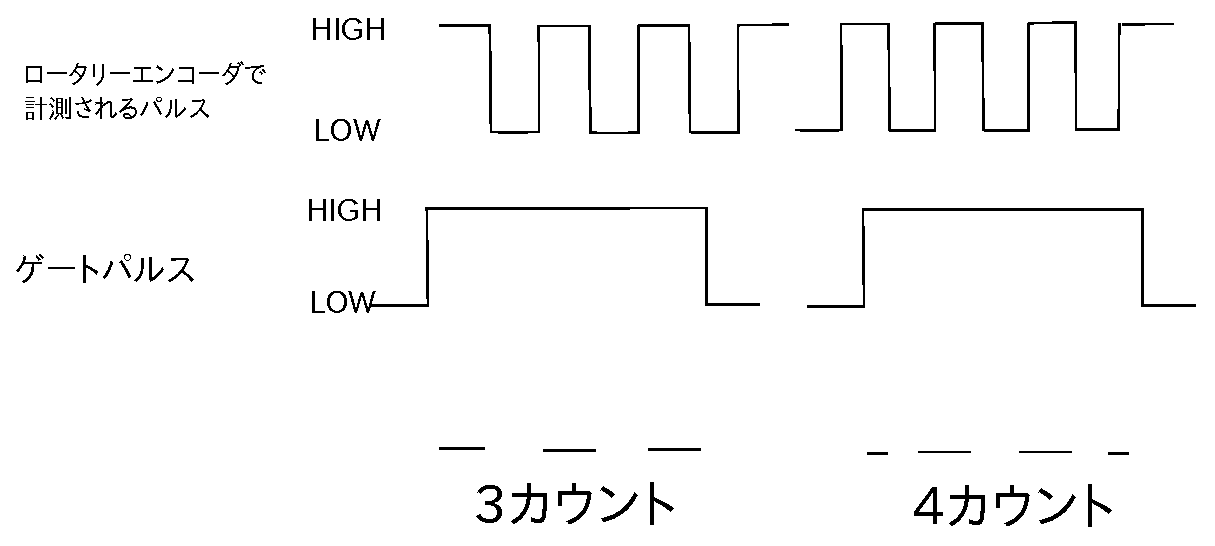
\includegraphics[width=12cm]{encoder.eps}
\end{center}
\caption{エンコーダカウント方式}
\end{figure}

\item 機械要素、制御要素による誤差
$\pm$1の誤差については、測定方法による誤差ということで説明がつくが、それ以上の誤差については測定対象であるマシニングセンタの誤差であると考えられる。このマシニングセンタでは、100$\sim$1000rpmはLowギヤ、1000$\sim$3000rpmはHighギヤで駆動する。100$\sim$1000rpmは誤差が$\pm$1の範囲に抑えられているが、1000$\sim$3000rpmでは誤差が$\pm$1の範囲外になってしまっているため、1rpm単位で設定できるこのマシニングセンタに誤差が生じていると考えられる。\\
\par
この誤差の理由について考えると、主軸回転の動力はDCモータが用いられている。DCモータはその構造上、電圧と回転数に線形性を持つ、という特性がある。おそらくDCモータの制御方法は、その線形性を利用してPWM制御を用いたオープンループ制御であると考えられる。こう考えると、回転数に比例して誤差が累積したという実験結果も説明がつく。よって、この誤差を抑えるには速度検出器を設置してフィードバックすれば良いと考えられる。例えばPID制御のような演算をして出力電圧を設定することで誤差は$\pm$1の範囲に収まると考えられる。
\end{itemize}
\subsubsection{回転数をアナログで計測する手法について以下のような検討をせよ}
\begin{enumerate}
\item アナログでの測定に用いる機器を採り上げなさい\\
ストロボスコープ\\
ストロボスコープを利用して回転数を計測する方法が存在する。これは、人間が見る残像効果を利用して計測する方法であるが、ビデオ等を用いて計測しデシタルで出力される製品も存在する。測定範囲は製品によるが10$\sim$100000rpm程で、高精度のものであれば読み取り値の$0.1\%$の精度が保証されている。\\
\item 誤差に表れる特徴をデジタル測定の場合と比較して考察せよ\\
回転数を上げるとそれに比例して精度を保証できないこのストロボスコープは、今回使用したロータリーエンコーダのデジタル化による誤差と比較すると測定精度は非常に悪いが、回転数の0.1\%の誤差が影響しても良いような大まかな速度を知りたいときには簡易的である。
\end{enumerate}
\subsection{ステージ送り}
\subsubsection{ステージ送り誤差}
\begin{enumerate}
\item アクチュエータにDCサーボモータを使用している点\\
DCサーボモータは電圧に比例して回転数が上がるDCモータの性質と正確な位置合わせができるサーボモータの性質を持っている。加えてサーボモータ自体がフィードバックの機構を持っているので、DCサーボモータを採用しているのは妥当である。
\item 送り要素にダブルナット方式ボールねじを利用している点\\
ダブルナット方式は与圧を両側にかけることで常に送り運動の動力をステージに伝えられる。正確な位置合わせとしては一般的に用いられている方法である。
\item 送り制御法としてモータ回転数をフィードバックしている点\\
モータの回転数だけでなく、位置を正確に測定できるセンサを設置してクローズドループにする方がより正確な位置決めが実現できる。
\item ダイヤルゲージのプローブの当て方による影響\\
今回の実験で採用したのは、回転式のレバー型プローブである。このプローブは直線運動を回転運動に変換し、角度を距離に直して測定している。このため直線式と比較すると誤差が生じやすい。

\begin{figure}[htbp]
\begin{center}
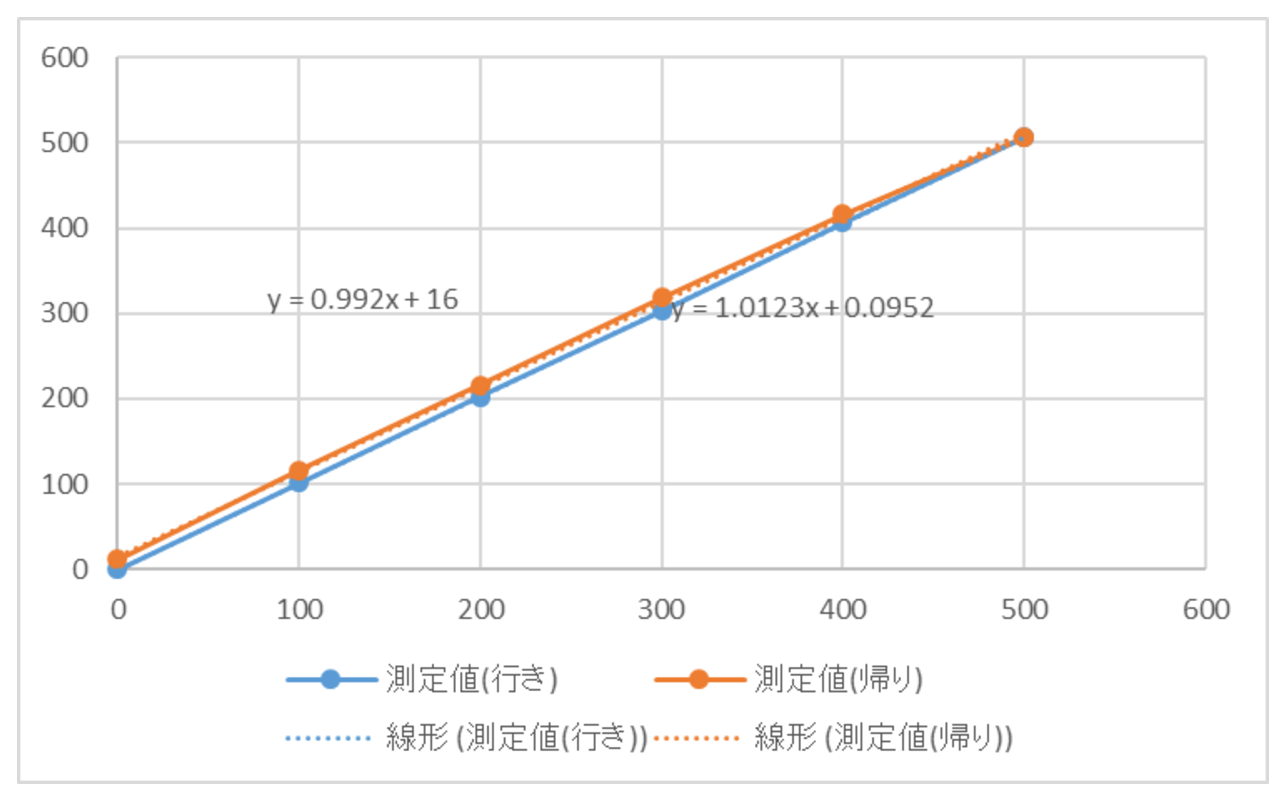
\includegraphics[width=12cm]{1.eps}
\end{center}
\caption{指定値と測定値の関係}
\end{figure}

2つの近似直線の傾きの平均を算出すると、
\begin{equation}
\alpha=(1.0123+0.992)/2=1.0575
\end{equation}

レバー式プローブのレバーの長さをr、初期角度をx、微小移動距離を$\delta$、微小変動角を$\Delta \theta$とすると、
\begin{eqnarray}
r\Delta \theta \cos x = \delta\\
r\Delta \theta = \delta \alpha\\
(2)を(3)で割ると、\nonumber\\
\cos x = \alpha\nonumber\\
x = \arccos \alpha
\end{eqnarray}

この計算により、初期速度は$x = 18.981 [degree]$と算出できる。

\item 実験で生じたヒステリシスについての考察\\
ダブルナットネジ方式を採用しているので、この分のバックラッシは非常に小さいものと考えられる。DCサーボモータはフィードバック機構によってバックラッシが補正されているものと考えると、ヒステリシスは部材の伸縮から来ているのではないかと考えられる。移動方向が変わると今までは圧縮力だったものが伸張力として作用し、伸張力が圧縮力として作用するので、10$\mu m$程の誤差が生じたと考えられる。
\end{enumerate}
\subsubsection{マシニングセンタの送り機構}
{\bf ラック&ピニオン式}

レールにラックギヤを設置して、ピニオンという歯車を組み合わせる送り機構。この方式はピニオンの回転数$\times$円周が移動距離という関係があるので、移動速度が速く、精度の良いものでは、単一ピッチ誤差が0.003[mm]、累積ピッチ誤差は500[mm]の移動で0.012[mm]程の精度実現が可能である。
\subsubsection{マシニングセンタの制御方法}
セミクローズドループ制御は、ロータリーエンコーダを用いた回転角検出を行い位置制御を行っているので、リニアエンコーダがなく簡易になるが、工作機械そのものに関係する誤差はフィードバックできない。そのためクローズドループ制御と比較すると精度は劣る。
\section{参考文献}
\begin{itemize}
\item 精密位置決め、送り系設計のための制御工学 松原厚\\
\item \url{http://www.nidec-shimpokeisoku.jp/products/05/}\\
\item 精密位置決め機構設計 工業調査会 大塚二郎ら
\end{itemize}
\end{document}